В библиотеке $\verb|pdpbox|$ представлены два типа графиков: для одного признака и для двух. Посмотрим на каждый:

\noindent
\begin{tabular}{c|c}
	\arrayrulecolor[rgb]{0.8,0.85,1}
	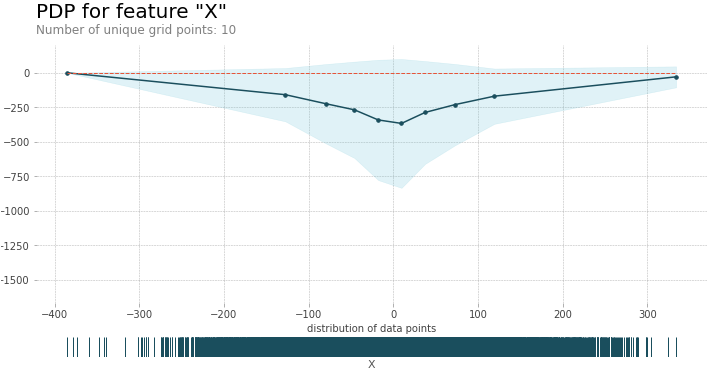
\includegraphics[width=0.48\linewidth]{pics/pdpx.png} & 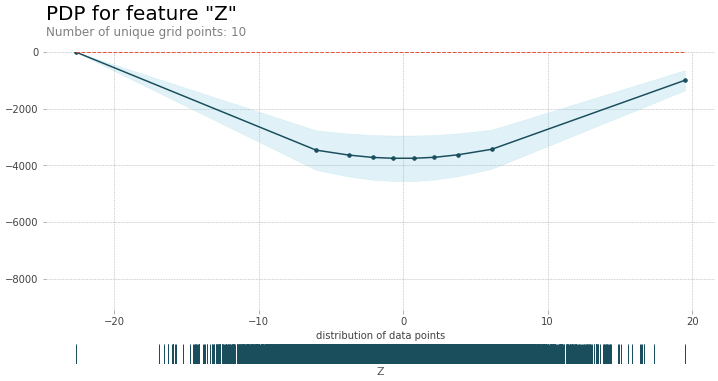
\includegraphics[width=0.48\linewidth]{pics/pdpz.png} \\
	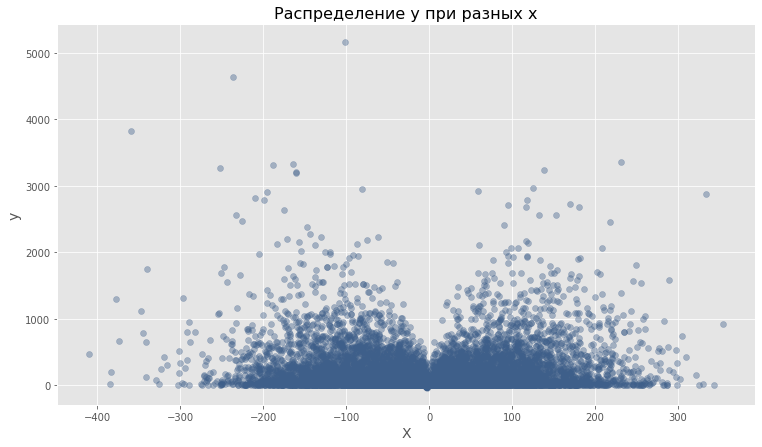
\includegraphics[width=0.48\linewidth]{pics/yx.png} & 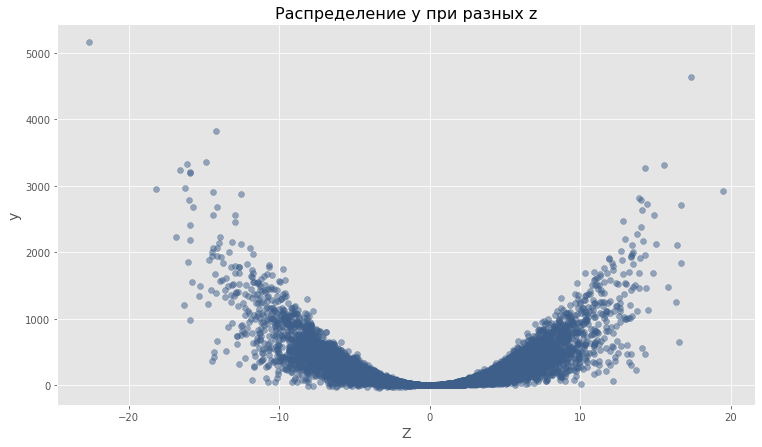
\includegraphics[width=0.48\linewidth]{pics/yz.png} \\
\end{tabular}

По графикам видно, что PDP действительно улавливает верную закономерность. Для признака $X$: PDP показывает углубление рядом с нулевым значениями, которое видно на данных. Аналогично, для признака $Z$: PDP показывает параболу, которая также хорошо заметна в выборке. Однако неточно отображен масштаб, эффект признака $X$ оказался занижен, признака $Z$ -- завышен. Это видно именно по PDP -- линии, показывающей эффект для среднего предсказания. Например, для $Z$ эффект $-4000$ не наблюдается практически ни для одного объекта. В целом PDP верно описывает закономерность в данных без учета масштаба.

Однако так получается не со всеми функциями. Рассмотрим небольшой контрпример:
\[
y = \frac{e^{-x^2-6x+5}}{70000} \cdot z - 3 \sin 0.3x + z^2
\]

\noindent
\begin{tabular}{c|c}
	\arrayrulecolor[rgb]{0.8,0.85,1}
	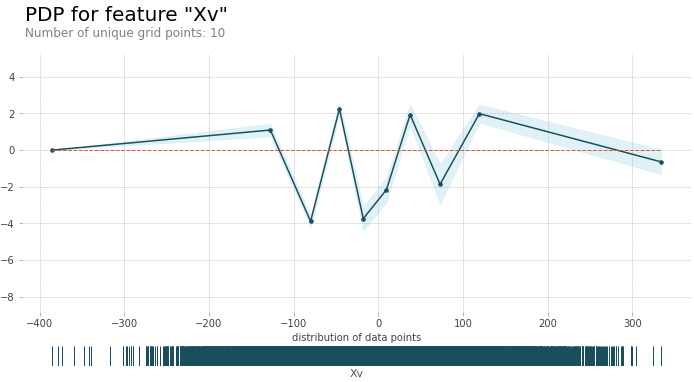
\includegraphics[width=0.46\linewidth]{pics/pdpce.png} & 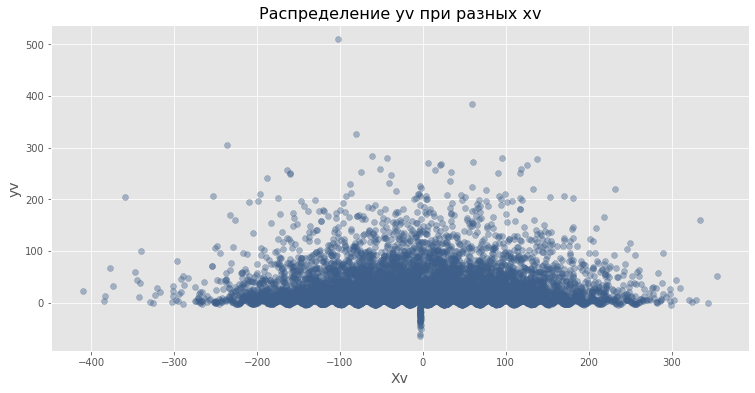
\includegraphics[width=0.5\linewidth]{pics/ce.png} \\
\end{tabular}

PDP показывает некоторые колебания эффекта переменной $Xv$ в интервале от $-100$ до $100$. И это может быть правдой в масштабе левого графика. Такие колебания можно заметить и на правом графике -- небольшие волны около нуля. Однако мы смотрим на выборку и видим более глобальную картину: чем ближе к нулю, тем больше эффект признака, хоть он и возрастает незначительно. Интуиция в данном случае конфликтует с результатом PDP -- стоит рассмотреть также другие точки зрения для принятия окончательных решений.

Вернемся к исходному примеру и взглянем на оба признака одновременно:

\noindent
\begin{tabular}{c|c}
	\arrayrulecolor[rgb]{0.8,0.85,1}
	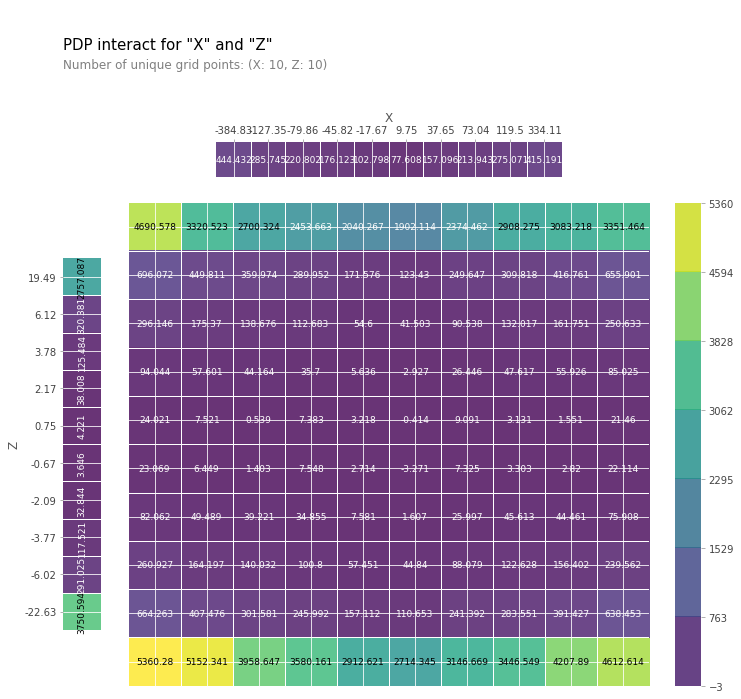
\includegraphics[width=0.5\linewidth]{pics/pdpxz1.png} & 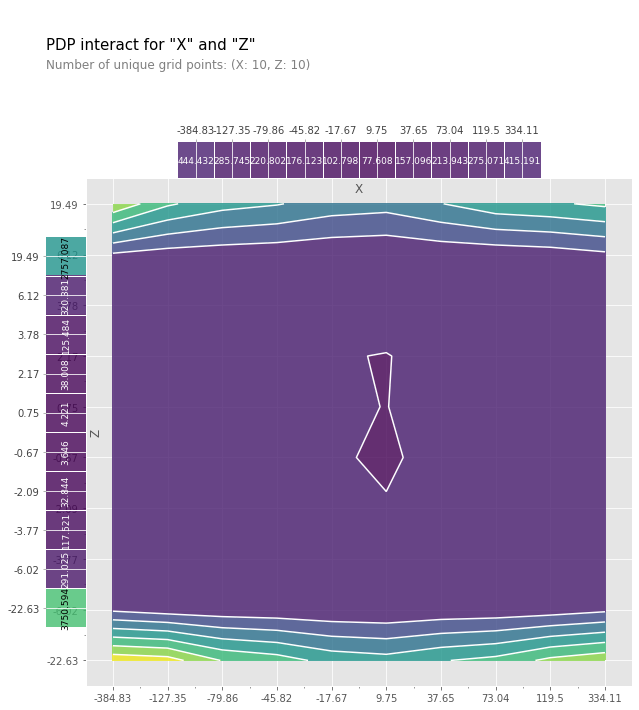
\includegraphics[width=0.42\linewidth]{pics/pdpxz2.png} \\
\end{tabular}

Получилась не очень показательная картинка. По ней кажется, что признак $X$ не оказывает особого влияния на результат. Данный график показывает не эффект признаков, а значение зависимой переменной. Поэтому вновь посмотрим на данные (возьмем масштаб побольше), чтобы сравнить PDP и истинную зависимость:

\begin{figure}[h]
	\centering{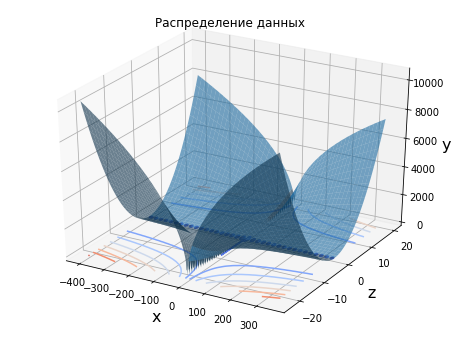
\includegraphics[width=0.6\linewidth]{pics/bigdata.png}}
\end{figure}

Получилось в самом деле похоже на истинную зависимость -- видно, по линиям уровня на 3D-графике.

PDP оказался довольно-таки хорош: он показал извлеченные из данных и модели зависимости, что полезно при анализе выборки и результатов работы модели. Однако стоит быть аккуратными -- контрпример показал, что не всегда PDP отображает то, что мы хотели бы получить.